\documentclass{beamer}
\mode<presentation>
{
  \usetheme{Warsaw}
  \definecolor{mcgarnet}{rgb}{0.38, 0, 0.08}
  \definecolor{mcgray}{rgb}{0.6, 0.6, 0.6}
  \setbeamercolor{structure}{fg=mcgarnet,bg=mcgray}
  %\setbeamercovered{transparent}
}


\usepackage[english]{babel}
\usepackage[latin1]{inputenc}
\usepackage{times}
\usepackage[T1]{fontenc}
\usepackage{tikz}
\usepackage{graphicx}

\newcommand{\imagesource}[1]{{\centering\hfill\break\hbox{\scriptsize Image Source:\thinspace{\small\itshape #1}}\par}}

\title{Even More Effective OOP Design}


\author{Robert Lowe\\}

\institute[Maryville College] % (optional, but mostly needed)
{
  Division of Mathematics and Computer Science\\
  Maryville College
}

\date[]{}
\subject{}

\pgfdeclareimage[height=0.5cm]{university-logo}{images/Maryville-College}
\logo{\pgfuseimage{university-logo}}



\AtBeginSection[]
{
  \begin{frame}<beamer>{Outline}
    \tableofcontents[currentsection]
  \end{frame}
}


\begin{document}

\begin{frame}
  \titlepage
\end{frame}

\begin{frame}{Outline}
  \tableofcontents
\end{frame}


% Structuring a talk is a difficult task and the following structure
% may not be suitable. Here are some rules that apply for this
% solution: 

% - Exactly two or three sections (other than the summary).
% - At *most* three subsections per section.
% - Talk about 30s to 2min per frame. So there should be between about
%   15 and 30 frames, all told.

% - A conference audience is likely to know very little of what you
%   are going to talk about. So *simplify*!
% - In a 20min talk, getting the main ideas across is hard
%   enough. Leave out details, even if it means being less precise than
%   you think necessary.
% - If you omit details that are vital to the proof/implementation,
%   just say so once. Everybody will be happy with that.

\section{Modelling Objects and Interactions}
\begin{frame}
    \frametitle{Object Diagrams}
    \begin{columns}
    \column{0.5\textwidth}
    \begin{itemize}[<+->]
        \item Object Diagrams capture object state during a specific
            time slice.
        \item Used in conjunction with use-case to capture objects.
        \item Basically like a class diagram, only it shows instances
            of objects.
        \item Often used to brainstorm for a class diagram.
    \end{itemize}
    \column{0.5\textwidth}
    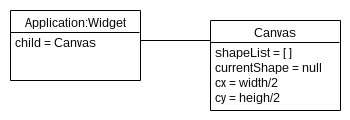
\includegraphics[width=\textwidth]{images/shapesObject}
    \end{columns}
\end{frame}

\begin{frame}
    \frametitle{Sequence Diagrams}
    \begin{itemize}[<+->]
        \item Sequence diagrams capture interactions between objects.
        \item There should be {\em at least} one sequence diagram per 
            Use-Case
        \item Activity diagrams are useful for identifying what methods an
            object needs to have.
        \item Often times you have additional sequence diagrams which 
            further explore internal operations of a system.
        \item The language consists of lifelines, process bars, actors,
            and objects.  
        \item Arrows indicate message passing, which in C++ corresponds to
            method calls.
    \end{itemize}
\end{frame}

\begin{frame}
    \frametitle{Sequence Diagrams}
    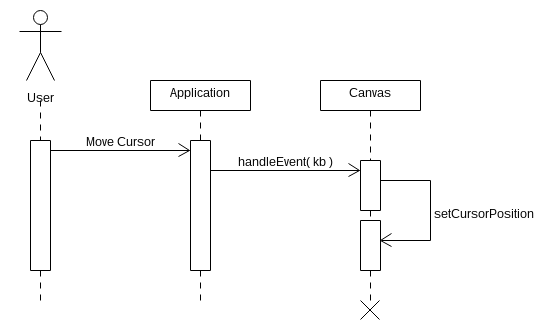
\includegraphics[width=\textwidth]{images/shapesActivity}
\end{frame}

\section{The Has..A Relationship}
\begin{frame}
    \frametitle{Aggregation}
    \begin{center}
        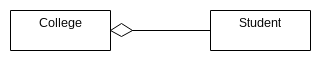
\includegraphics[height=0.2\textheight]{images/aggregation}
    \end{center}
    \begin{itemize}[<+->]
        \item Aggregation is a generic ``has-a'' relationship.
        \item It is also referred to as ``weak composition''
        \item Here, an object is composed of several otherwise independent
            objects.
        \item Classic examples are employees to companies,
            students to schools, or ducks to ponds.
        \item Aggregation is represented by a line with an empty diamond
            on the side of the aggregate object.
        \item Aggregation can appear on both object and class diagrams.
    \end{itemize}
\end{frame}

\begin{frame}
    \frametitle{Composition}
    \begin{center}
        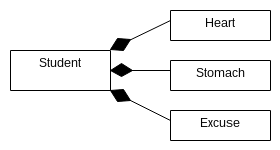
\includegraphics[height=0.3\textheight]{images/composition}
    \end{center}
    \begin{itemize}[<+->]
        \item Composition is a stronger ``has-a'' relationship.
        \item In composition, the composite object is responsible for
            the creation and maintenance of the subordinate objects.
        \item Composition is represented by a filled in diamond on the
            composite class.
    \end{itemize}
\end{frame}

\section{End-to-End Process}
\begin{frame}
    \frametitle{Detailed, Buzz-Word Compliant, OO Process}
    \begin{enumerate}[<+->]
        \item Gather requirements.
        \item Generate a use case diagram.
        \item Using the use case diagram, generate an object diagram.
        \item Generate sequence diagrams for all your use cases.
        \item Using your object and sequence diagrams, create a class diagram.
        \item Identify commonalities between classes, create abstract 
            classes as needed.
        \item Identify and mark aggregations and compositions.
        \item Write your code (if you still have time).
    \end{enumerate}
\end{frame}

\begin{frame}
    \frametitle{Pong Revisited}
    Let's build on what we did last time to fully specify Pong.  
    If we have time, we'll even implement it!
    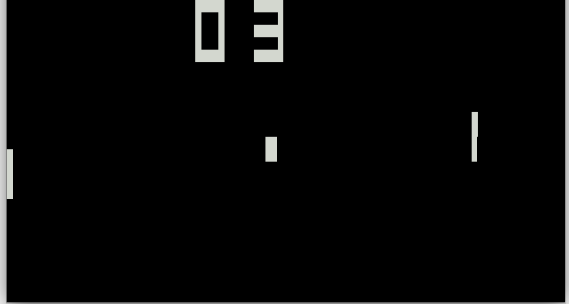
\includegraphics[width=\textwidth]{images/pong}
\end{frame}
\end{document}